\scanpage{285}
\[
\uline{\operatorname{Pic}}_{X/S}^{\tau}\simeq\uline{\operatorname{Pic}}_{Y/S}^{\tau}\times A'^{\Gamma}
\]
-- Par exemple, prenant $\Gamma=\mathbb Z/2\mathbb Z$, \inserted{opérant sur $A$ par symétrie,} $B$ un autre schéma abélien, sur lequel $\Gamma$ opère par translation par une section qui est partout d'ordre $2$ exactement (i.e. on a un isom de $\Gamma_S\longrightarrow B$) -- de sorte que $Y$ est également un schéma abélien sur $S$ -- alors
\[
\uline{\operatorname{Pic}}_{X/S}^{\tau}\simeq Y'\times {}_2 A'
\]
On notera que $\uline{\operatorname{Pic}}_{X/S}^{\tau}$ est \uline{plat} sur $S$.
En caractéristiques résiduelles $\ne 2$, $\uline{\operatorname{Pic}}_{X/S}^{\tau}$ est \unsure{$=$} \deleted{\unsure{séparé}} \uline{simple} sur $S$. Mais il ne l'est pas en un pt $s\in S$ de car. résiduelle $2$.
C'est l'exemple de \uline{Igusa}. [N.B. On peut prendre pour $A,B$ des \uline{courbes} elliptiques, donc $X$ est une \uline{surface}. \deleted{\unsure{Cela étant} \illegible{1}, on peut supposer} \uline{On notera que} $H^1(X,\unsure{\uline{\mathcal O}|\mathcal O}_X)$ \uline{est de dimension} égale à
\[
\dim B+\dim A
\]
alors que $\dim\uline{\operatorname{Pic}}_{X/\unsure{k|K}}=\dim B$. On notera que l'exemple ne donne pas de ``saut'' pour le $H^1(X,\unsure{\uline{\mathcal O}|\mathcal O}_X)$ en \unsure{égales} caractéristiques. Dans cet exemple, $\uline{\operatorname{Pic}}_{X/S}^{\tau}$ admet
\figure{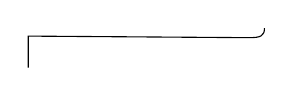
\begin{tikzpicture}\draw (0,0)--(0,0.4)--(2.8,0.38)..controls (2.95,0.38) and (3,0.4)..(3,0.5);\end{tikzpicture}}
\mspage{284}
